\section{Results}

\subsection{Eye tracking accuracy requirements}
\label{sec:accuracy_results}

\begin{figure}[b]
    \centering
    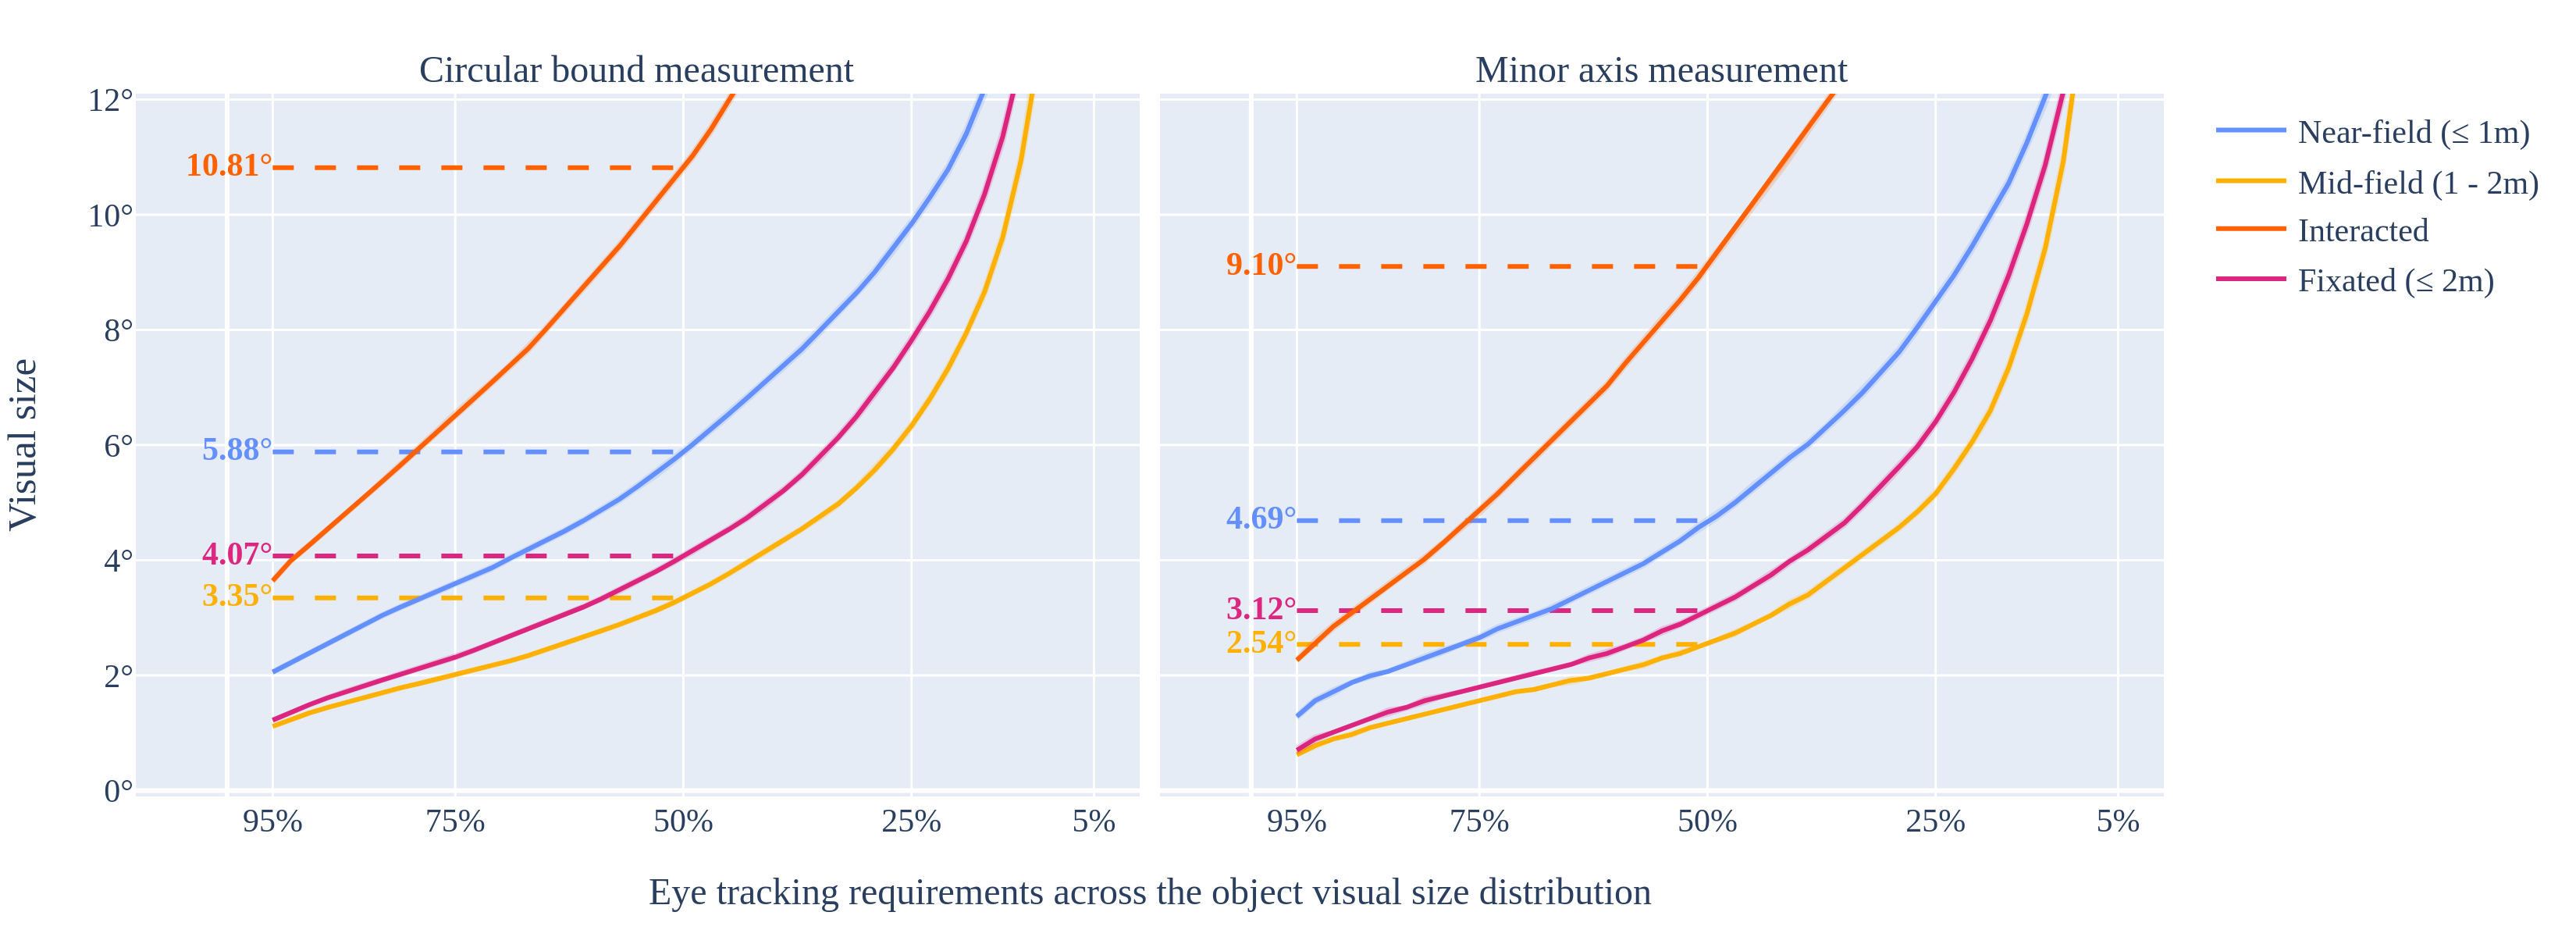
\includegraphics[width=\linewidth]{figures/vis_size.png}
    \caption{Eye tracking accuracy requirements to place gaze accurately within in the ADT dataset, where users performed household actions in an indoor environment~\cite{pan_adt_2023}  Near-field and mid-field measurements consider all objects present in the user's field of view, where interacted objects are being actively manipulated by the user, and fixated objects consider those being directly gazed at.}
    \label{fig:visual_sizes}
\end{figure}

The \textbf{near-field} ($\leq$ 1 meter) and \textbf{mid-field} (1 - 2 meters) measurements reflect the visual FOV occupied by \textit{every} object in the environment within the distance threshold.  Alternatively, the \textbf{interacted} measurement only aggregates objects when being manually interacted with, including picking up, pushing, pressing, etc.  \textbf{Fixation} measurements consider the objects within 2 meters at the time of fixation.  Considering ADT's household scenarios, the \textbf{interacted} and \textbf{fixation} categories reflect the distribution of objects likely to be of interest during daily tasks.

To estimate ET accuracy requirements, we computed the entire distribution of object visual sizes recorded in camera projection space. To place gaze on an object of average (projected) size 50\% of the time, we measure at the distribution's 50\% mark.  These measurements can help to inform system design; while 50\% reliability may be \textit{useful supporting context} in a broader contextual AI agent, a system relying heavily on ET may aim for higher coverage.  The distributions for each interaction scenario are seen in \autoref{fig:visual_sizes}.

Recall that we use angular \textbf{radius} to represent the \textbf{average case} ET requirements, and \textbf{minor axis} span as a more \textbf{conservative} measurement.  The accuracy of wearable ET devices is known to suffer in dynamic conditions~\cite{onkhar_tobii_2023}, yet recent devices remain quite accurate in unconstrained settings\footnote{\url{https://www.tobii.com/products/eye-trackers/wearables/tobii-pro-glasses-3}}\footnote{\url{https://pupil-labs.com/products/neon}}.  Assuming a device with $\leq 3 \degree$ accuracy during daily wear, our results indicate that the majority of fixated objects (radius average=$4.07\degree$; minor axis=$3.12\degree$), the majority of objects in the near-field (radius=$5.88\degree$; minor axis=$4.69\degree$), and nearly all interacted objects (radius=$10.81\degree$; minor axis=$9.10\degree$) are reliable for placing gaze on the correct object.  Conversely, objects in the mid-field (radius=$3.3\degree$; minor axis=$2.54\degree$) will be somewhat unreliable at this signal quality, where roughly half of objects are not able to be detected.

\subsection{Contextualized vision-language model queries}
\label{sec:vlm_queries}

\begin{figure}[t]
    \centering
    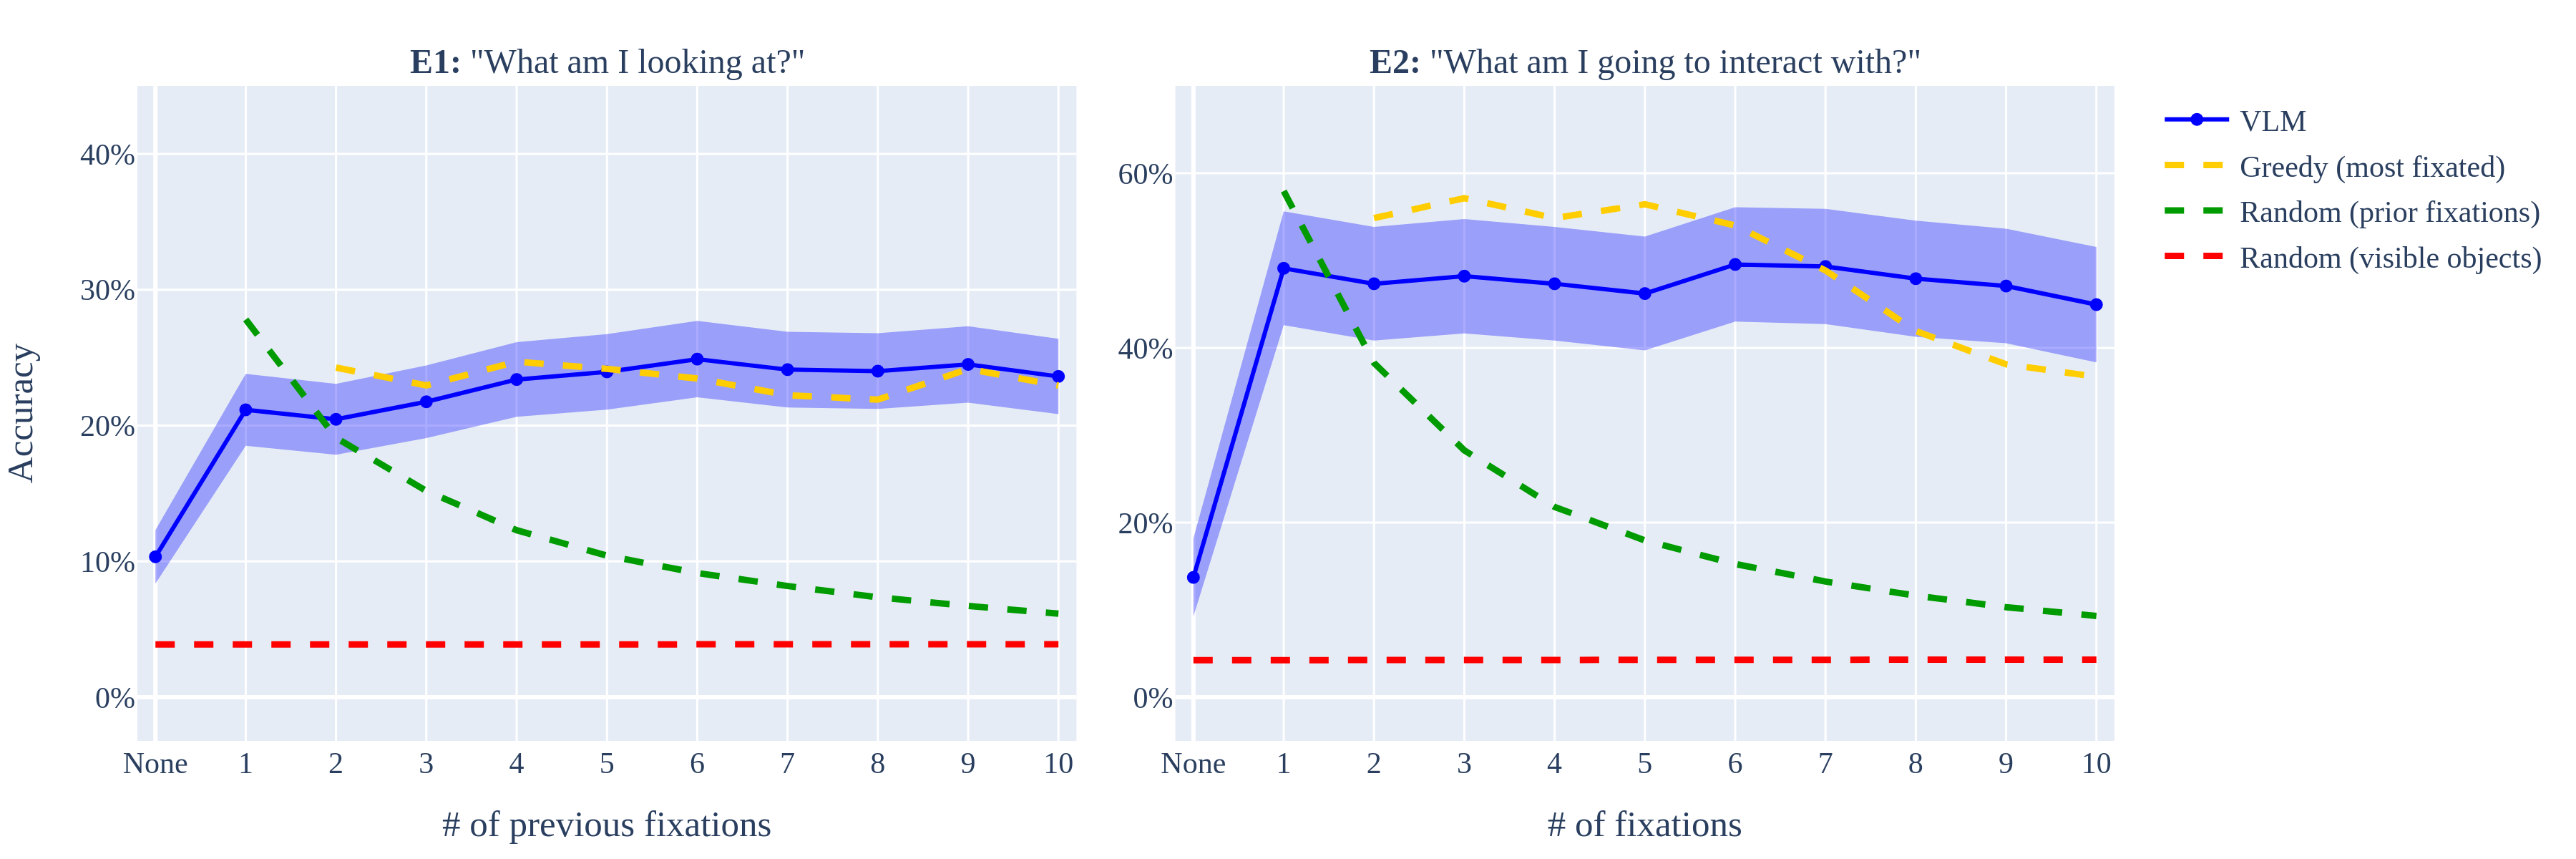
\includegraphics[width=\linewidth]{figures/e1e2.png}
    \caption{Experiments where prior gaze fixation contents are supplied to a VLM along with egocentric images.  When many fixations given as context, the model can synthesize information between the image + gaze context to outperform a greedy baseline that only considers contents from the prompt. The error surfaces in light blue represent 95\% confidence intervals.}
    \label{fig:e1e2}
\end{figure}

Because we constrain the VLM model to respond by selecting from the list of all currently visible objects, these experiments are classification tasks where \textit{accuracy = correct selections / all trials}.  Cases where the VLM response failed to return parseable JSON ($<$1\% of trials) were discarded.

We compare against a number of baselines to see if the model effectively uses the context supplied.  These baselines implement simple heuristics on the image and gaze context.  The lowest performing baseline is random guessing among all visible objects.  We also implement random guesses from the list of previously fixated objects, and a greedy strategy which always chooses the most fixated object from a sequence of previously fixated objects.  Note these baselines still use context provided from ET, but make no attempt to synthesize with the egocentric image for better world understanding.

\subsubsection{E1: ``What am I looking at?"}

When querying the VLM only with the egocentric image as context, the model successfully predicts the current fixated object 10.3\% (95\% CI = [8.3\%, 12.3\%]) of the time (see \autoref{fig:e1e2} (left)).  While this surpasses random guessing from visible objects, it is quite low.  An effective strategy was to always return the immediately preceding fixation (left tail of Random (prior fixations) in \autoref{fig:e1e2}).  VLMs are not expected to excel at gaze prediction, as they are known to misinterpret context or hallucinate~\cite{cui_holistic_2023, leng_hallucinations_2024}.  However, including context from prior gaze greatly improves the model's ability to predict the current fixation, with a peak accuracy of 24.8\% (CI = [22.1\%, 27.7\%]) at 6 prior fixations.  The gaze context-based baselines slightly outperform the VLM with one or few prior fixations, reinforcing that current gaze is contingent on scanpath history~\cite{burlingham_laziness_2024, burlingham_scanpaths_2024}.  With more context (6+ fixations), the model begins to outperforms baselines, indicating that prior context and image contents are being synthesized, and the combination of contextual cues increase the model's performance.

\subsubsection{E2: ``What am I going to interact with?"}

E2 sees similar trends to E1; however, the more contextually-grounded task to predict the object of physical interaction sees greater benefit when including ET context. Clearly, prior eye gaze is a strong indicator for interaction, and by supplying historical gaze context, we can greatly improve the VLM's ability to understand the user's actions. We see a peak accuracy of 49.5\% (CI = [43\%, 56.1\%]). As evident by this and the stronger baseline performances, gaze is tightly coupled with the onset of interaction. Note that we query only at positive examples where an interaction does take place, and the inclusion of a null case could have led to the model raising false positives / negatives.


% \subsubsection{E3: Gaze-based context cropping}

% \NOTE{Holding space for this experiment.} \lipsum[1] \lipsum[2]